\documentclass[border=3pt]{standalone}
\usepackage{tikz}
\usetikzlibrary{calc}
\begin{document}
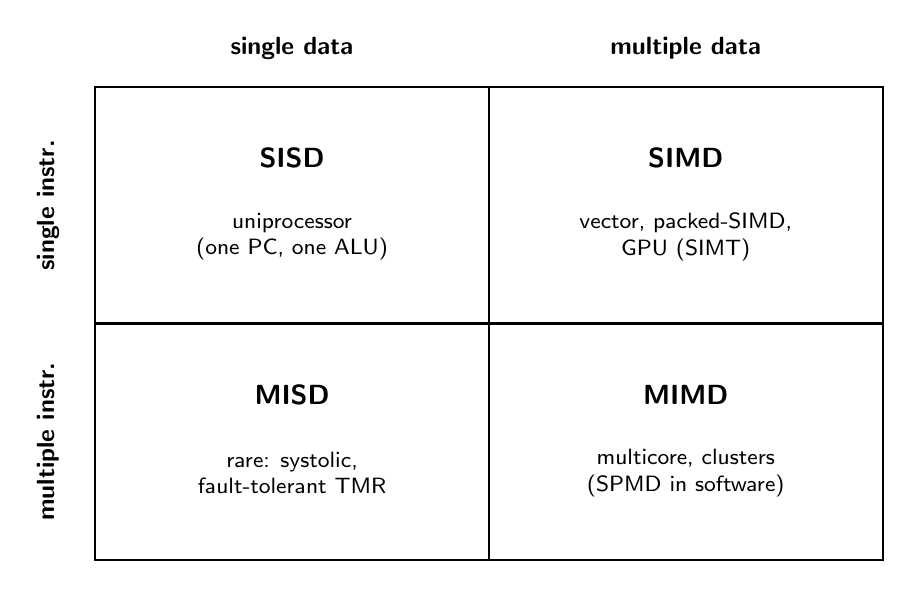
\begin{tikzpicture}[font=\sffamily\small, x=1mm, y=1mm]
  % 2x2 grid
  \draw[thick] (0,0) rectangle (100,60);
  \draw[thick] (50,0) -- (50,60);
  \draw[thick] (0,30) -- (100,30);
  % axis labels
  \node[font=\sffamily\small\bfseries, rotate=90] at (-6,45) {single instr.};
  \node[font=\sffamily\small\bfseries, rotate=90] at (-6,15) {multiple instr.};
  \node[font=\sffamily\small\bfseries] at (25,65) {single data};
  \node[font=\sffamily\small\bfseries] at (75,65) {multiple data};
  % quadrants
  \node[font=\sffamily\bfseries] at (25,51) {SISD};
  \node[align=center, font=\sffamily\footnotesize] at (25,41) {uniprocessor\\(one PC, one ALU)};
  \node[font=\sffamily\bfseries] at (75,51) {SIMD};
  \node[align=center, font=\sffamily\footnotesize] at (75,41) {vector, packed-SIMD,\\GPU (SIMT)};
  \node[font=\sffamily\bfseries] at (25,21) {MISD};
  \node[align=center, font=\sffamily\footnotesize] at (25,11) {rare: systolic,\\fault-tolerant TMR};
  \node[font=\sffamily\bfseries] at (75,21) {MIMD};
  \node[align=center, font=\sffamily\footnotesize] at (75,11) {multicore, clusters\\(SPMD in software)};
\end{tikzpicture}
\end{document}
